\documentclass{beamer}
\mode<presentation> 
\usetheme{CambridgeUS}
\usecolortheme{seagull}
%\setbeamertemplate{headline}
%\setbeamertemplate{footline} 
% To remove the footer line in all slides uncomment this line

%\setbeamertemplate{footline}[page number] 
% To replace the footer line in all slides with a simple slide count uncomment this line

\setbeamertemplate{navigation symbols}{} 
% To remove the navigation symbols from the bottom of all slides uncomment this line

\usepackage{graphicx}
\usepackage{booktabs} 
\usepackage[round]{natbib}
\usepackage{verbatim}
\usepackage{subfigure}
\usepackage{multicol}
\newcommand{\beginbackup}{
	\newcounter{framenumbervorappendix}
	\setcounter{framenumbervorappendix}{\value{framenumber}}
}
\newcommand{\backupend}{
	\addtocounter{framenumbervorappendix}{-\value{framenumber}}
	\addtocounter{framenumber}{\value{framenumbervorappendix}} 
}
%----------------------------------------------------------------------
%	TITLE PAGE
%----------------------------------------------------------------------

\title[Narrative Conservatism]{Narrative Conservatism} % The short title appears at the bottom of every slide, the full title is only on the title page
\author[]{Juan Manuel Garc\'ia Lara, Beatriz Garc\'ia Osma, Fengzhi Zhu} % Your name
\institute[] % Your institution as it will appear on the bottom of every slide, may be shorth and to save space
{Universidad Carlos III de Madrid \\ % Your institution for the title page

	\medskip
	fzhu@emp.uc3m.es} % Your email address
\date{\today} % Date, can be changed to a custom date (\today)

\begin{document}
	
\begin{frame}
\titlepage % Print the title page as the first slide
\end{frame}

%-----------------------------------------------------------------
\begin{frame}
\frametitle{Outline}
\tableofcontents
\end{frame}

%-------------------------------------------------------------------
%	PRESENTATION SLIDES
%----------------------------------------------------
\section{Research Question and Contribution}
%------------------------------------------------

\begin{frame}
\frametitle{Research Question and Contribution}
\begin{itemize}
\item \textbf{Research Question}

\begin{itemize}
\item Whether narrative disclosure is conservative, i.e., whether narratives reflect bad news in a more complete, news-consistent, and timely manner than good news?
\end{itemize}

\item \textbf{Contribution}

\begin{itemize}
	\item Filling the gap in conservatism literature by documenting the existence of narrative conservatism.
	\item Providing novel evidence to the debate regarding whether managers withhold bad news. 
	\item Relating to the broader literature on the informativeness of SEC filings.
\end{itemize}
\end{itemize}
\end{frame}
%------------------------------------------------
\section{Theoretical Framework}
%------------------------------------------------
\begin{frame}
\frametitle{Theoretical Framework: Recognition and Disclosure}
\begin{itemize}
\item \textbf{Definition \citep{schipperRequiredDisclosuresFinancial2007}}
	
	\begin{itemize}
		\item Recognition: depictions in numbers with captions on the face of the financial statements
		\item Disclosure: display in the notes and supporting schedules that accompany financial statements
	\end{itemize}

\item \textbf{Reporting Requirement \citep{fasbStatementFinancialAccounting1984}}

	\begin{itemize}
		\item Recognition: an economic event can be recognized if it satisfies all of the following criteria
		\begin{itemize}
			\item Definition criterion
			\item Measurability criterion
			\item Relevance criterion
			\item Reliability criterion
		\end{itemize}
	% First, the item must meet the definition of an element of financial statements (definition criterion). Second, the item must have a relevant attribute measurable with sufficient reliability (measurability criterion). Third, the information about the item must be capable of making a difference in user decisions (relevance criterion). Fourth, the information must be representationally faithful, verifiable, and neutral (reliability criterion).
		\item Disclosure: can be deployed to disclose information that fails to meet certain recognition criteria
	\end{itemize}

\item \textbf{Role of Narratives} 

	\begin{itemize}
		\item Supplement information that cannot be recognized
		\item Explain recognized line items
	\end{itemize}

\end{itemize}
\end{frame}
%------------------------------------------------
\begin{frame}
\frametitle{Theoretical Framework: Conservatism}
\begin{itemize}
		
\item \textbf{Definition}

	\begin{itemize}
		\item Conditional conservatism: ``accountants' tendency to require a higher degree of verification to recognize good news as gains than to recognize bad news as losses" \citep*[p. 7]{basuConservatismPrincipleAsymmetric1997}
		\item Unconditional conservatism: ``accountants' preference for accounting methods that lead to lower reported values for shareholders' equity" \citep*[p. 8]{basuConservatismPrincipleAsymmetric1997}.
		\item Narrative conservatism: narratives reflecting bad news in a more complete, news-consistent and timely manner than good news
	\end{itemize}

\end{itemize}
\end{frame}
%------------------------------------------------
\begin{frame}
	\frametitle{Theoretical Framework: Completeness}
	\begin{itemize}
\item \textbf{Completeness}

\begin{itemize}
	\item Complete disclosure must include all necessary information for a user to understand the underlying economic event \citep{fasbConceptualFrameworkFinancial2018}
	\item Firms may disclose good news in a more complete manner than bad news to boost performance \citep{teohEarningsManagementUnderperformance1998, langVoluntaryDisclosureEquity2000}.
	\item Firms may disclose bad news in a more complete manner than good news to avoid litigation \citep{skinnerWhyFirmsVoluntarily1994, skinnerEarningsDisclosuresStockholder1997}.
\end{itemize}

\item \textbf{Hypotheses}

\begin{itemize}
	\item  \textbf{H1:} Narrative disclosure is completer in response to bad news than to good news.
\end{itemize}

\end{itemize}
\end{frame}
%------------------------------------------------
\begin{frame}
	\frametitle{Theoretical Framework: News-consistency}
	\begin{itemize}
		\item \textbf{News-consistency}
		
		\begin{itemize}
			\item News-consistency implies that disclosure agrees with the underlying economic event in content sentiment. %Specifically, we interpret it as the degree to which firms use positive tone in narrative disclosure in response to good news and negative tone in response to bad news.
			\item Tone influences how information is perceived or processed, and thus it can be employed both to inform or mislead \citep{davisNumbersMeasuringInformation2012, liInformationContentForwardLooking2010, huangToneManagement2014}.
			\item Firms may deploy a uniformly positive (negative) tone in both good and bad news disclosure, resulting in higher news-consistency in good (bad) news disclosure.
		\end{itemize}
		
		\item \textbf{Hypotheses}
		
		\begin{itemize}
			\item  \textbf{H2}: Narrative disclosure is more news-consistent in response to bad news than to good news.
		\end{itemize}
		
	\end{itemize}
\end{frame}
%------------------------------------------------
\begin{frame}
	\frametitle{Theoretical Framework: Timeliness}
	\begin{itemize}
		\item \textbf{Timeliness}
		
		\begin{itemize}
			\item Financial information is of higher quality if it is \textit{timely}. Disclosure should be made \textit{in time} to influence users' decisions \citep{fasbConceptualFrameworkFinancial2018}.
			\item Managers may delay bad news disclosure to mitigate its negative economic consequences \citep{chambersTimelinessReportingStock1984, niessnerStrategicDisclosureTiming2015, segalAreManagersStrategic2016, brockbankStrategicTiming8K2018}.
			\item Managers may accelerate bad news disclosure due to litigation concerns \citep{skinnerWhyFirmsVoluntarily1994, marinovicNoNewsGood2016}.
		\end{itemize}
		
		\item \textbf{Hypotheses}
		
		\begin{itemize}
			\item  \textbf{H3}: Narrative disclosure is timelier in response to bad news than to good news.
		\end{itemize}
		
	\end{itemize}
\end{frame}
%------------------------------------------------
%\begin{frame}
%	\frametitle{Theoretical Framework: Conservatism Continued}
%	\begin{itemize}
%
%\item \textbf{Is conservatism useful?}
%
%	\begin{itemize}
%		\item Valuation role: provide financial information about the reporting entity that is useful to existing and potential investors, lenders, and other creditors in making decisions about providing resources to the entity \citep[OB2]{fasbConceptualFrameworkFinancial2018b}
%		\item Stewardship role: how efficiently and effectively the entity's management and governing board have discharged their responsibilities to use the entity's economic resources \cite[OB4]{fasbConceptualFrameworkFinancial2018b}
%	\end{itemize}
%
%\item \textbf{Is narrative conservatism useful?}
%	\begin{itemize}
%		\item We posit that narrative conservatism enhances contract efficiency and serves the stewardship role of accounting
%		\item Testable hypotheses to be developed
%	\end{itemize}
%
%\end{itemize}
%\end{frame}
%%------------------------------------------------
\section{Research Design}
%------------------------------------------------
\begin{frame}
\frametitle{Research Design: Proxies}
\begin{itemize}

\item \textbf{Narrative Disclosure Corpora}

	\begin{itemize}
		\item Corpora: 10-Q and 8-K filings because they (a) are more credible, (b) have higher reporting threshold and (c) are more timely than other corporate communication channels.
		\item Heterogeneity between 10-Q and 8-K: (a) 10-Q is more diversified in content (b) 8-K is more timely.
	\end{itemize}

\item \textbf{Proxies for Textual Properties and News}
	\begin{itemize}
		\item Completeness: the total number of words of SEC filings
		\item News-consistency: the marginal change of tone in response to increase (good news) or decrease (bad news) in stock market returns.
		\item Timeliness: reporting time lag, defined as the number of days elapsed between the news release date and the filing date of the studied disclosure
		\item News: stock returns \citep{basuConservatismPrincipleAsymmetric1997}.
	\end{itemize}

\end{itemize}
\end{frame}
%------------------------------------------------
\begin{frame}
	\frametitle{Research Design: Model}
	\begin{itemize}

\item \textbf{Model Specification}
	\begin{itemize}
		\item Form 10-Q
		
		\begin{figure}[h]
			\centering
			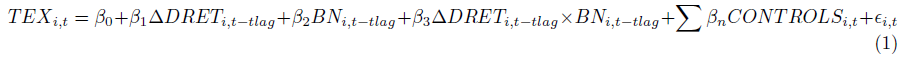
\includegraphics[width=0.75\linewidth]{eq1}
			\label{eq1}
		\end{figure}
	
		\item Form 8-K
		
		\begin{figure}[h]
			\centering
			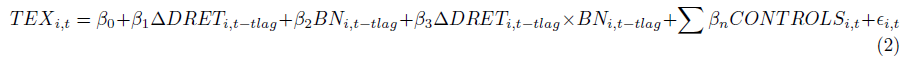
\includegraphics[width=0.8\linewidth]{eq2}
			\label{eq2}
		\end{figure}
	
		\begin{figure}[h]
			\centering
			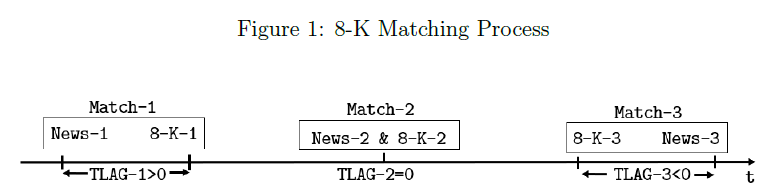
\includegraphics[width=0.6\linewidth]{fig1}
			\label{fig1}
		\end{figure}
	\end{itemize}

\end{itemize}
\end{frame}
%------------------------------------------------
\begin{frame}
\frametitle{Research Design: Data}

\begin{itemize}
	\item Data source: Compustat, CRSP and I/B/E/S
	
	\begin{figure}[h]
		\centering
		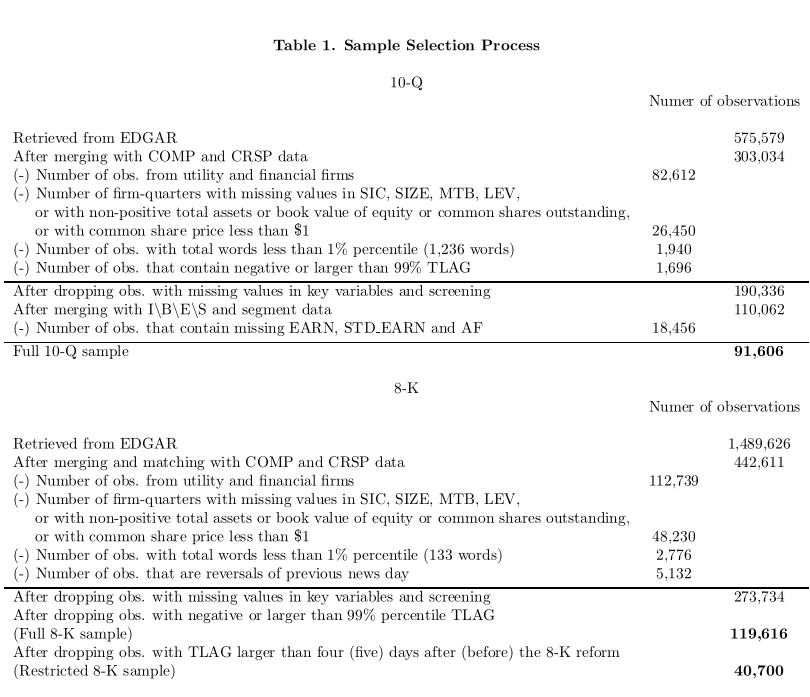
\includegraphics[width=0.65\linewidth]{tab1}
		\label{tab1}
	\end{figure}

\end{itemize}
\end{frame}
%------------------------------------------------
\section{Results}
%------------------------------------------------
\begin{frame}
\frametitle{Results: Summary Statistics}
\begin{figure}[h]
	\centering
	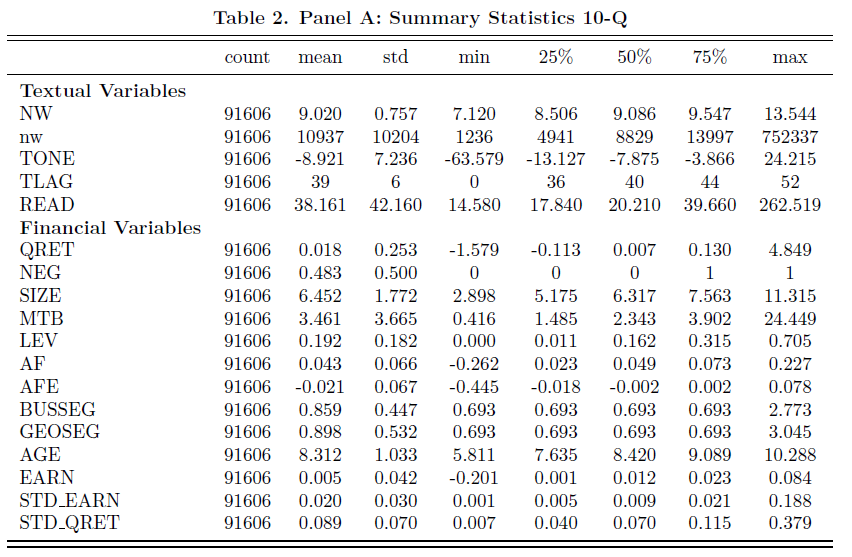
\includegraphics[width=0.65\linewidth]{tab2panA}
	\label{tab2panA}
\end{figure}

\end{frame}
%------------------------------------------------
\begin{frame}
	\frametitle{Results: Summary Statistics Continued}
	\begin{figure}[h]
		\centering
		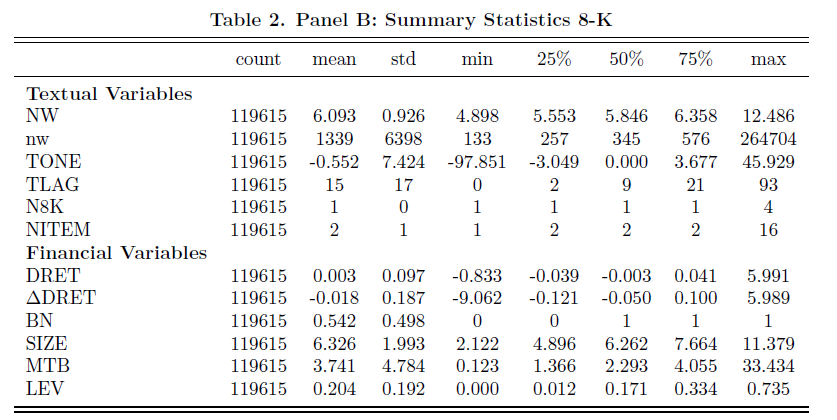
\includegraphics[width=0.65\linewidth]{tab2panB}
		\label{tab2panB}
	\end{figure}
	
\end{frame}
%------------------------------------------------
\begin{frame}
	\frametitle{Results: Summary Statistics Continued}
	\begin{figure}[h]
		\centering
		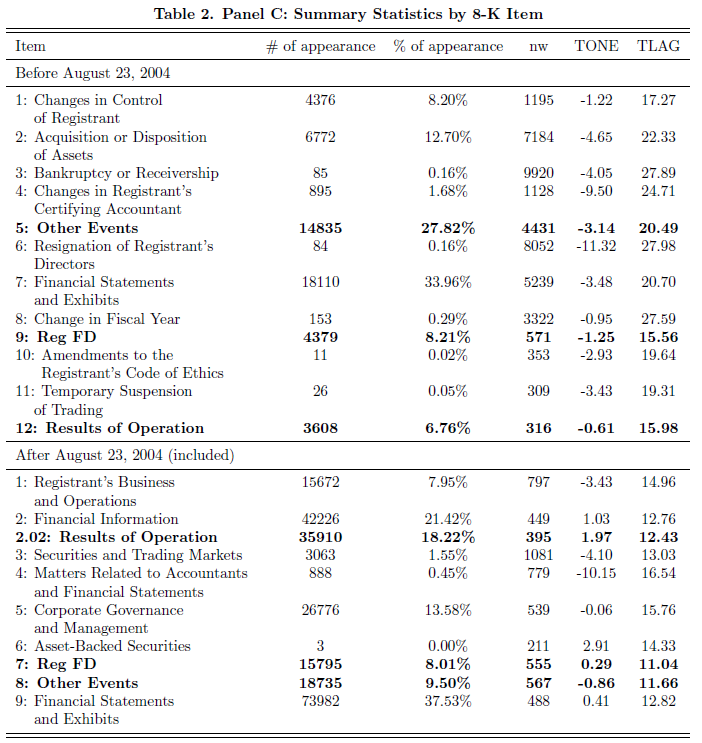
\includegraphics[width=0.55\linewidth]{tab2panC}
		\label{tab2panC}
	\end{figure}
	
\end{frame}
%------------------------------------------------
\begin{frame}
\frametitle{Results: Is 10-Q Narrative Disclosure Conservative?}
	\begin{figure}[h]
		\centering
		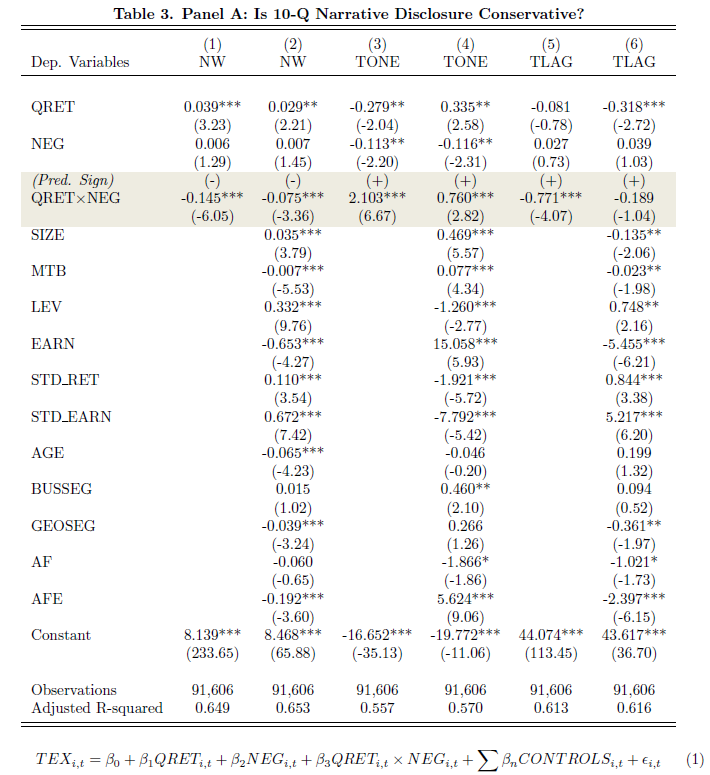
\includegraphics[width=0.55\linewidth]{tab3panA}
		\label{tab3panA}
	\end{figure}
\end{frame}
%------------------------------------------------
\begin{frame}
\frametitle{Results: Are Lengthier 10-Qs Less Readable?}
	\begin{figure}[h]
	\centering
	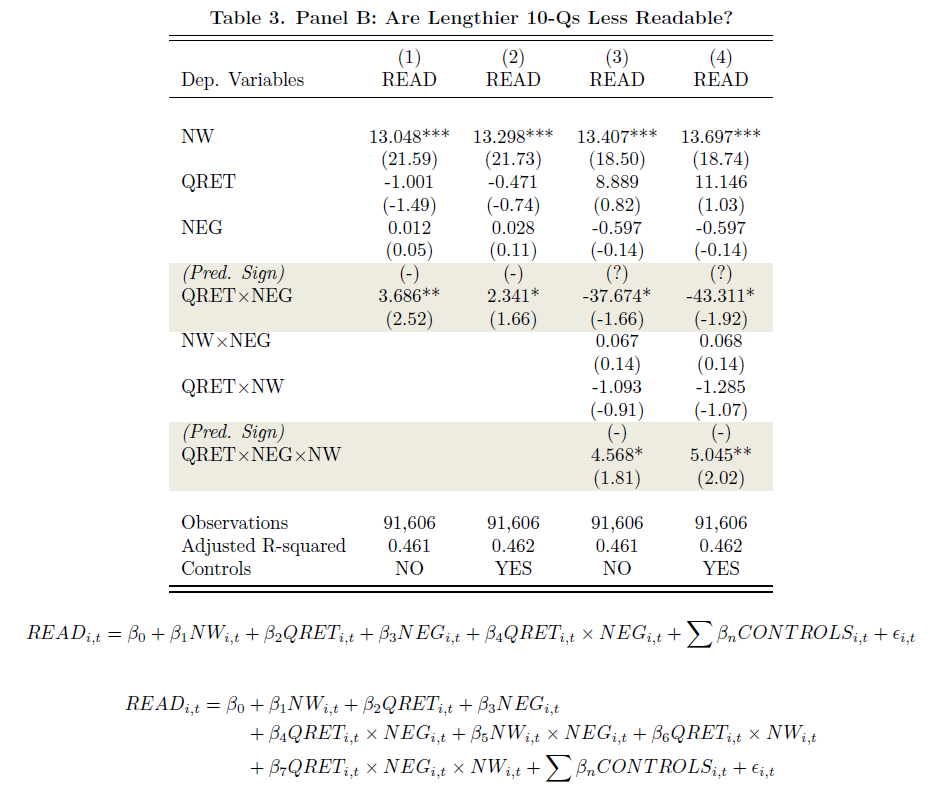
\includegraphics[width=0.75\linewidth]{tab3panB}
	\label{tab3panB}
	\end{figure}
\end{frame}
%------------------------------------------------
\begin{frame}
\frametitle{Results: Is 8-K Narrative Disclosure Conservative?}
	\begin{figure}[h]
	\centering
	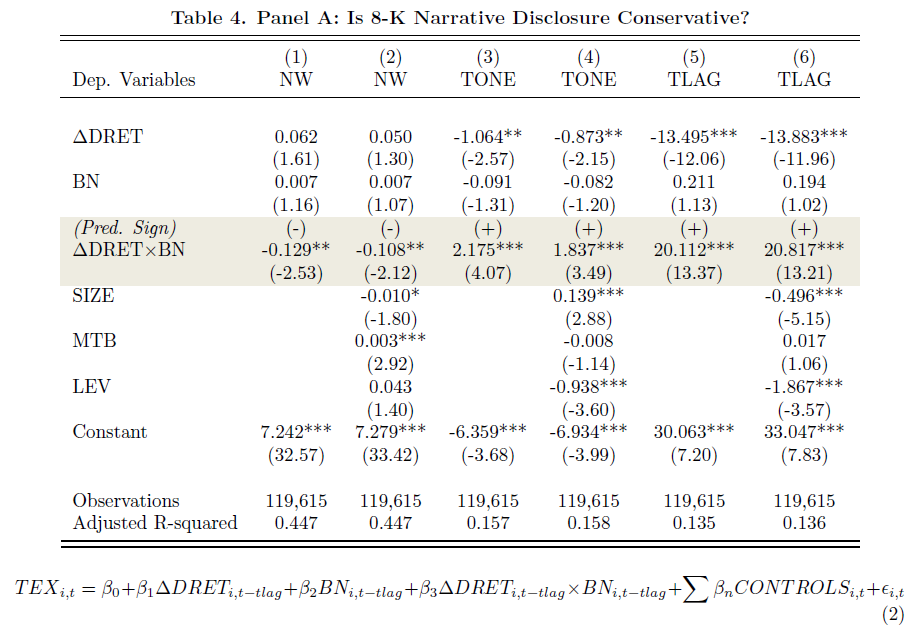
\includegraphics[width=0.7\linewidth]{tab4panA}
	\label{tab4panA}
	\end{figure}
\end{frame}
%------------------------------------------------
\begin{frame}
\frametitle{Results: 8-K Items, Filings and Reporting Time Lag}
	\begin{figure}[h]
	\centering
	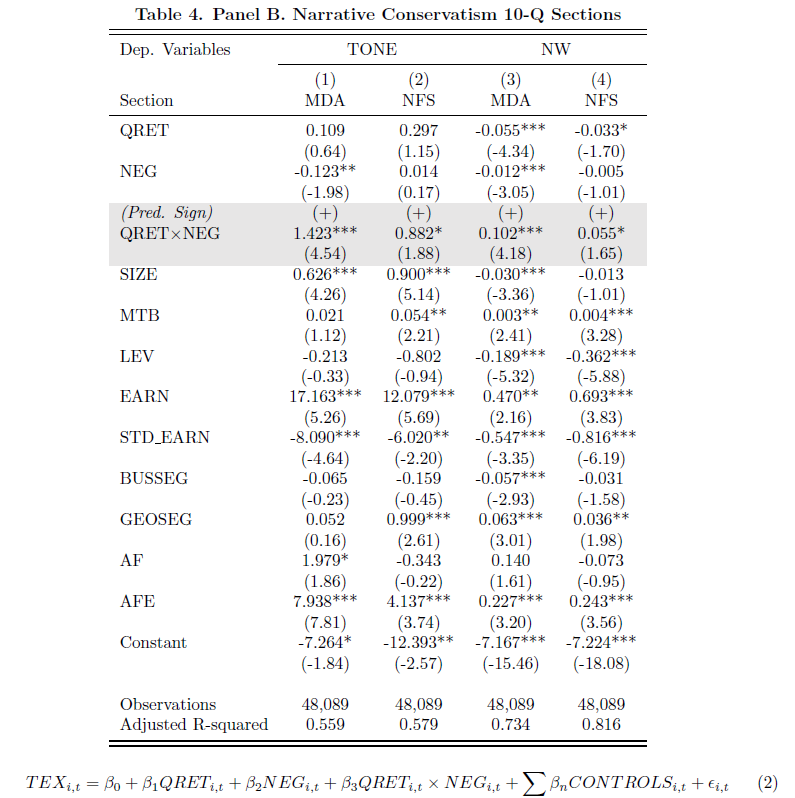
\includegraphics[width=0.65\linewidth]{tab4panB}
	\label{tab4panB}
	\end{figure}
\end{frame}
%------------------------------------------------
\begin{frame}
	\frametitle{Results: Robustness Checks}
\begin{itemize}
	\item Our evidence of narrative conservatism is robust to 
	\begin{itemize}
		\item employing an alternative tone measure using the positive and negative word list from the Harvard General Inquiry dictionary \citep{loughranTextualAnalysisAccounting2016};
		\item including controls for conditional conservatism and managerial incentives;
		\item excluding 8-K items on results of operations that contain quarterly or annual financial statements \citep{segalAreManagersStrategic2016};
		\item using an alternative 8-K reporting time lag definition \citep{carterRelevanceForm8K1999, niessnerStrategicDisclosureTiming2015, chapmanInformationOverloadDisclosure2019};
		\item excluding a priori bad news 8-K items \citep{segalAreManagersStrategic2016};
		\item estimating by fiscal year from 1995 to 2020.
	\end{itemize}
\end{itemize}
\end{frame}
%------------------------------------------------
\section{Additional Analyses}
%------------------------------------------------
\begin{frame}
\frametitle{Additional Analyses: MD\&A and NFS}
	\begin{figure}[h]
	\centering
	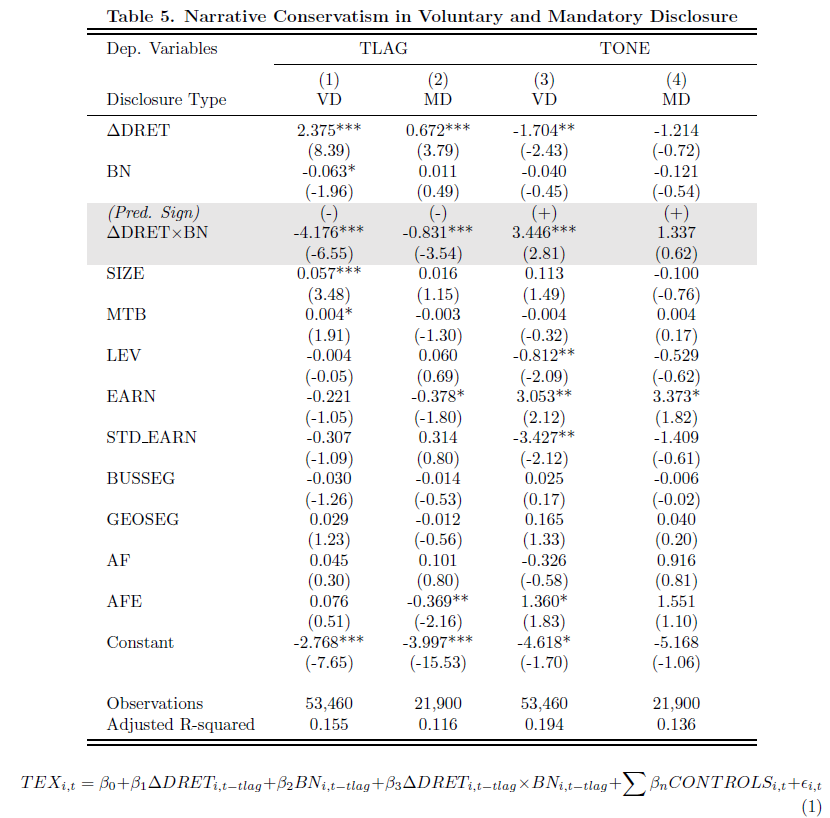
\includegraphics[width=0.58\linewidth]{tab5}
	\label{tab5}
	\end{figure}
\end{frame}
%------------------------------------------------
\begin{frame}
\frametitle{Additional Analyses: Voluntary and Mandatory Disclosure}
	\begin{figure}[h]
	\centering
	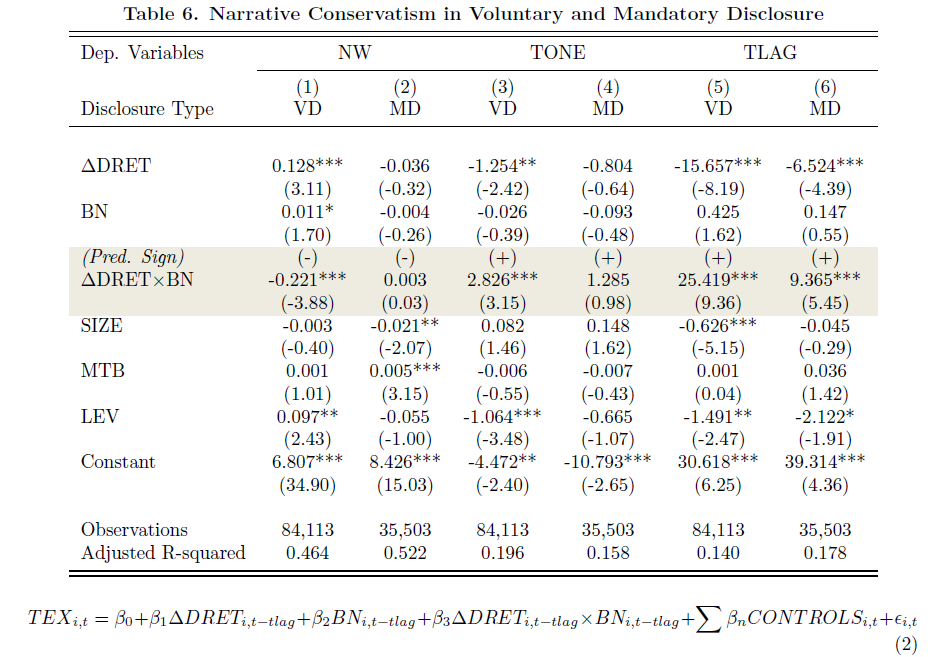
\includegraphics[width=0.7\linewidth]{tab6}
	\label{tab6}
	\end{figure}
	
\end{frame}
%------------------------------------------------
\begin{frame}
	\frametitle{Additional Analyses: Intangible Assets and R\&D Expenses}
	\begin{figure}[h]
	\centering
	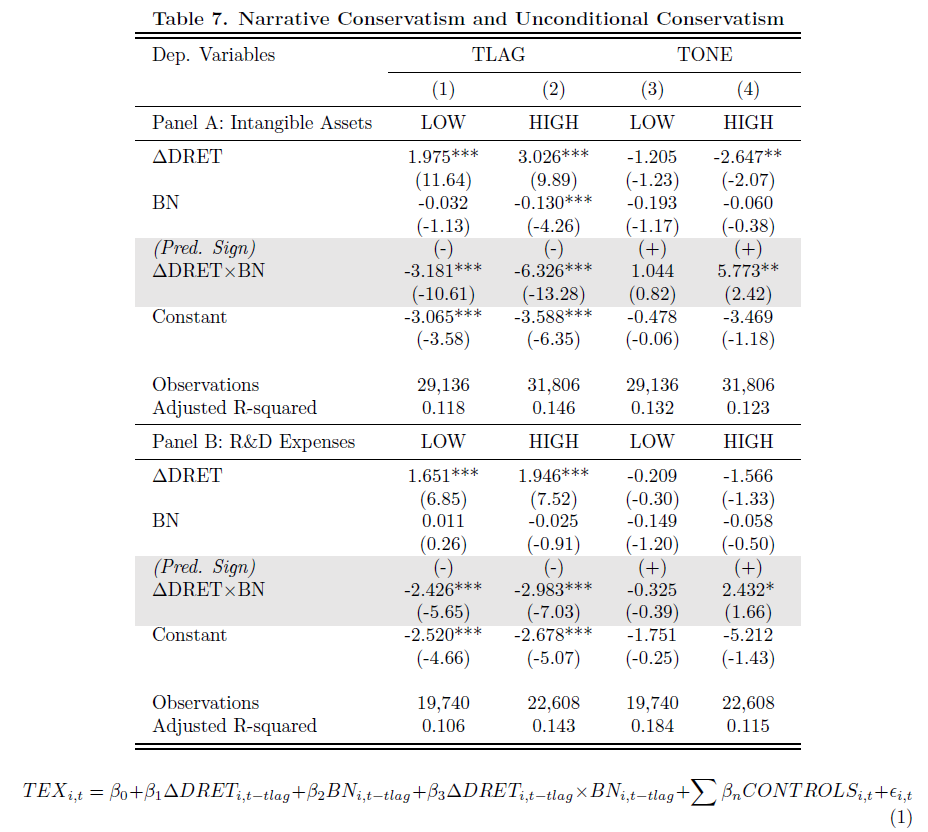
\includegraphics[width=0.7\linewidth]{tab7}
	\label{tab7}
	\end{figure}
	
\end{frame}
%------------------------------------------------
\begin{frame}
	\frametitle{Additional Analyses: Firm Characteristics}
	\begin{figure}[h]
		\centering
		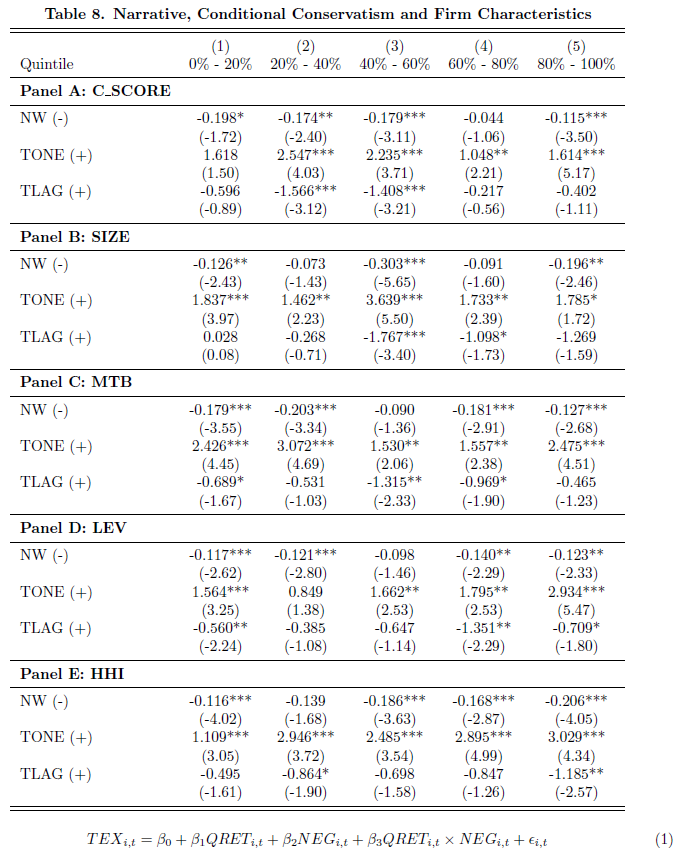
\includegraphics[width=0.5\linewidth]{tab8}
		\label{tab8}
	\end{figure}
	
\end{frame}
%------------------------------------------------
\begin{frame}
	\frametitle{Additional Analyses: Managerial Incentives}
	\begin{figure}[h]
	\centering
	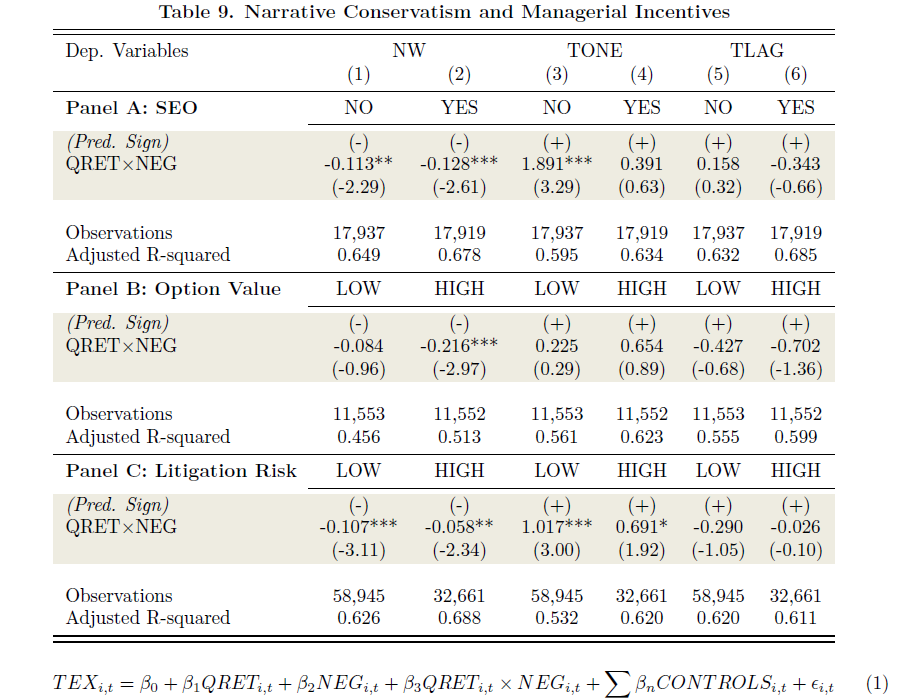
\includegraphics[width=0.7\linewidth]{tab9}
	\label{tab9}
	\end{figure}
\end{frame}
%------------------------------------------------
\section{Conclusions}
%------------------------------------------------
\begin{frame}
\frametitle{Conclusions}
\begin{itemize}
	\item \textbf{Conclusions}
	\begin{itemize}
		\item We provide evidence that narratives reflect bad news in a more complete, news-consistent, and timely manner than good news. 
		\item Firms report lengthier 10-Qs to clarify rather than obfuscate bad news, and provide more 8-Ks and 8-K items in response to bad news than to good news.
		\item We document greater narrative conservatism in the MD\&A section and in voluntary disclosure. Also, narrative conservatism is pervasive in firms with high conditional conservatism, intangible assets, R\&D expenses and proprietary costs.
		\item We find greater narrative conservatism in settings where managers have strong incentives to disclose bad news.
	\end{itemize}

	\item \textbf{Future Research}
	\begin{itemize}
		\item An aggregate measure of narrative conservatism
		\item Economic implications of narrative conservatism
		\item Mechanisms that assure the credibility of narrative conservatism 
	\end{itemize}
	
\end{itemize}

\end{frame}
%------------------------------------------------
\section{References}
%------------------------------------------------
\beginbackup
\begin{frame}<presentation:0>
\frametitle{Selected References}
\scriptsize
\bibliographystyle{plainnat}
\bibliography{NC_slides}
\end{frame}
\backupend
%------------------------------------------------
\end{document}